\documentclass[12pt]{article}
\newcommand{\pdftitle}{periodic-boundary-conditions}
\input{preamble}


\newcommand{\ustar}{u^{\ast}}

\pagestyle{fancy}
\fancyhead[L]{Periodic Boundary Conditions}
\fancyhead[C]{}
\fancyhead[R]{E. Torres}
\renewcommand{\headrulewidth}{1.0pt}
\fancyfoot[L]{\today}
\fancyfoot[C]{}
\fancyfoot[R]{\thepage}
\renewcommand{\footrulewidth}{1.0pt}

\begin{document}
\section{Finite difference equations for $u^{\ast}$ velocity}
Starting with a figure highlighting the cell centered periodic boundary
conditions in light red, we can write the following $\ustar$ equations:
\begin{itemize}
    \item Left boundary (i.e., $i=1/2$ coding index \texttt{u(:,0)})
        \begin{subequations}
            \begin{equation}
                \begin{aligned}
                    u^{\ast}_{\frac{1}{2},j} = u^{n}_{\frac{1}{2},j} & -  \Delta t\Bigg[ 
                    \frac{
                        \big(u^{n}_{1,j}\big)^{2} - \big(u^{n}_{-1,j}\big)^{2}
                    }{\Delta x} +
                    \frac{
                        \left(uv\right)^{n}_{\frac{1}{2},j+\frac{1}{2}} - \left(uv\right)^{n}_{\frac{1}{2},j-\frac{1}{2}}
                    }{\Delta y}
                    \Bigg]\\
                    & + \Delta t \Bigg[
                        \frac{
                            u^{n}_{\frac{3}{2},j} - 2u^{n}_{\frac{1}{2},j} + u^{n}_{M+\frac{1}{2},j}
                        }{\Delta x^{2}}
                     + 
                        \frac{
                            u^{n}_{\frac{1}{2},j+1} - 2u^{n}_{\frac{1}{2},j} + u^{n}_{i+\frac{1}{2},j-1}
                        }{\Delta y^{2}}
                        \Bigg]
                \end{aligned}
            \end{equation}
            \text{where} 
            \begin{equation}
                u^{n}_{-1,j} = \frac{1}{2} \left(u^{n}_{1/2,j} + u^{n}_{M+1/2,j} \right)
            \end{equation}
        \end{subequations}
    \vspace{0.1in}
    \item Interior points (i.e., $i=\frac{3}{2}$ through $i=M-1/2$ coding index \texttt{u(:,1:M-1)})
        \begin{equation}
            \begin{aligned}
                u^{\ast}_{i+\frac{1}{2},j} = u^{n}&_{i+\frac{1}{2},j}  -  \Delta t\Bigg[ 
                \frac{
                    \big(u^{n}_{i+1,j}\big)^{2} - \big(u^{n}_{i-1,j}\big)^{2}
                }{\Delta x} +
                \frac{
                    \left(uv\right)^{n}_{i+\frac{1}{2},j+\frac{1}{2}} - \left(uv\right)^{n}_{i+\frac{1}{2},j-\frac{1}{2}}
                }{\Delta y}
                \Bigg]\\
                & + \Delta t \Bigg[
                    \frac{
                        u^{n}_{i+\frac{3}{2},j} - 2u^{n}_{i+\frac{1}{2},j} + u^{n}_{i-\frac{1}{2},j}
                    }{\Delta x^{2}}
                 + 
                    \frac{
                        u^{n}_{i+\frac{1}{2},j+1} - 2u^{n}_{i+\frac{1}{2},j} + u^{n}_{i+\frac{1}{2},j-1}
                    }{\Delta y^{2}}
                    \Bigg]
            \end{aligned}
        \end{equation}
    \vspace{0.1in}
    \item Right boundary (i.e., $i=M+1/2$ coding index \texttt{u(:,M)})
        \begin{subequations}
            \begin{equation}
                \begin{aligned}
                    u^{\ast}_{M+\frac{1}{2},j} = &u^{n}_{M+\frac{1}{2},j}  -  \Delta t\Bigg[ 
                    \frac{
                        \big(u^{n}_{M+1,j}\big)^{2} - \big(u^{n}_{M,j}\big)^{2}
                    }{\Delta x} +
                    \frac{
                        \left(uv\right)^{n}_{M+\frac{1}{2},j+\frac{1}{2}} - \left(uv\right)^{n}_{M+\frac{1}{2},j-\frac{1}{2}}
                    }{\Delta y}
                    \Bigg]\\
                    & + \Delta t \Bigg[
                        \frac{
                            u^{n}_{\frac{1}{2},j} - 2u^{n}_{M+\frac{1}{2},j} + u^{n}_{M-\frac{1}{2},j}
                        }{\Delta x^{2}}
                     + 
                        \frac{
                            u^{n}_{M+\frac{1}{2},j+1} - 2u^{n}_{M+\frac{1}{2},j} + u^{n}_{M+\frac{1}{2},j-1}
                        }{\Delta y^{2}}
                        \Bigg]
                \end{aligned}
            \end{equation}
            \text{where}
            \begin{equation}
                u^{n}_{M+1,j} = \frac{1}{2} \left(u^{n}_{M+\frac{1}{2}} + u^{n}_{\frac{1}{2}} \right)
            \end{equation}
        \end{subequations}
\end{itemize}
\section{Finite difference equations for $v^{\ast}$ velocity}
\section{Finite difference equations for $p$}
\begin{figure}[H]
    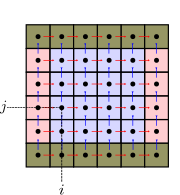
\includegraphics[height=0.5\textheight]{../../../media/periodic-BCs}
    \caption{Cell center periodic domain}
    \label{fig:periodic-domain}
\end{figure}                                                            

\section{Testing results}
\subsection{Poiseuille's flow}
The following is for the center line velocity profile for a Poiseuille flow
simulation.
\begin{figure}[H]
    \includegraphics[height=0.5\textheight]{../data/data-64-dev/u-poiseuille.png}
    \caption{Cell center periodic domain}
    \label{fig:periodic-domain}
\end{figure}                                                            

\end{document}
